\documentclass{40k}

\usepackage{pdflscape}

%%----------------------------------------------------------------------
%% Deployment Zones
%%----------------------------------------------------------------------

\newcommand{\dephammerandanvil}%
{Deployment zones are \textbf{Hammer and Anvil}, as defined on
  page~131 of the main rulebook (24'' short edges).}

\newcommand{\vanguardstrike}%
{Deployment zones are \textbf{Vanguard Strike}, as defined on page~131
  of the main \emph{Warhammer 40,000} rulebook.  Vanguard Strike may
  be approximated by deploying within a 33.5'' x 50'' table corner
  triangle.  The player that wins the zone roll off may pick any of
  the four corners, and the other player takes that diagonally
  opposite.}

\newcommand{\quartered}%
{Deployment zones are the rectangles in each table corner~12'' in from
  the long edge and~24'' in from the short edges.  The player that
  wins the zone roll off picks either pair of \emph{diagonally
    opposite} corners as their deployment zone and a long table edge
  as their player edge.  The other player takes the other pair of
  diagonally opposite corners and opposite long edge.}

%%----------------------------------------------------------------------
%% Secondaries
%%----------------------------------------------------------------------


%%----------------------------------------------------------------------
%% Secondaries
%%----------------------------------------------------------------------

\newcommand{\seekanddestroy}%
{\item \textit{Seek and Destroy.}  Choose and declare a Battlefield
  Role other than Troop.  Score~2 victory points for each enemy unit
  of this role completely destroyed or falling back at the end of the
  game.}

\newcommand{\seizeground}%
{\item \textit{Seize Ground.}  Choose two terrain pieces not in your
  deployment zone.  Do not declare these now, but do secretly record
  your selection unambiguously!  Reveal these at game end and score~3
  victory points for each piece that you control, treating them as
  objective markers.  Note that this means a single unit cannot claim
  both a primary objective marker and a terrain piece simultaneously.}

\newcommand{\reconnaissance}%
{\item \textit{Reconnaissance.}  At the end of the game, score~2
  victory points for each friendly scoring unit with the Scout or
  Infiltrate USR completely within 12'' of your opponent's table
  edge.}

\newcommand{\meatgrinder}%
{\item \textit{Meatgrinder.}  Score~1 victory point for each opposing
  Troop unit completely destroyed or falling back at the end of the
  game.}

\newcommand{\assassination}%
{\item \textit{Assassination.}  Score~1 victory point for each
  opposing character model removed as a casualty or falling back at
  the end of the game.  Note that this is not limited to just
  independent characters.}

\newcommand{\controlthefield}%
{\item \textit{Control the Field.}  Each table quarter in which you
  have a scoring unit and your opponent does not, or you have an
  Objective Secured Unit and your opponent does not, is worth 2
  victory points.}


%%----------------------------------------------------------------------
%% Tertiaries
%%----------------------------------------------------------------------

\newcommand{\tertiaries}%
{\missionsubheading{Tertiary Objectives.}
  As given in the overall Common Rules section of this packet.}


%%----------------------------------------------------------------------
%%----------------------------------------------------------------------
\begin{document}

\pagetitle{Mission Pack}

\begin{columns}

\missionheading{Army Construction}

Armies must be selected to at most~\underline{1850 points}.

Players will use a single army list for all missions.  All up to date
sources\footnote{Partial list maintained by Redcap's Corner and PAGE:
  \url{http://bit.ly/1uWkFHz}} are permitted.  No requirements or
constraints are placed on detachments or force organizations.  Forge
World units and armies eligible for standard \emph{Warhammer 40,000}
are permitted.

Models need not be painted, but objective painting scores will be
applied to reward finished armies.

Models must be WYSIWYG, but identifiable and thoughtful conversions
are welcome.  Contact the tournament organizer(s) beforehand about any
uncertain models.  ``Counts-as'' proxies and undistinguishable or
confusing stand-ins are not permitted.

\missionheading{Supporting Materials}

You must have an official, legal, complete physical or digital copy on
hand for all army, unit, and other sources you are using.  You should
bring printed copies of relevant pages of any electronic sources.
Don't forget errata and FAQs for your sources.\footnote{Available from
  Games Workshop:
  \url{http://www.games-workshop.com/Rules-Errata}}

You must bring any dice, templates, and markers you need to facilitate
playing your army, as well as five typed copies of your army roster
with points listed.

%\vfill
%\begin{story}{62pt}{The Shift}
%\end{story}
%\columnbreak

\missionheading{Scoring}%

Match results are determined by scoring primary, secondary, and
tertiary objectives as given for each mission.  The winner is the
player with more victory points at game end.  The players draw if they
have earned equal victory points.  No more than~20 victory points may
be earned per mission toward the standings, though any additional
victory points do count toward determining match results.

Pure competition standings, i.e., the Best General prize(s) if
awarded, are determined first by win/draw/loss records and then the
sum total victory points earned across all three missions.

Overall tournament rankings and the primary prize(s) are based on
points earned toward a maximum of~100 available for the day:
\begin{itemize}\shortlist
\item 60 points for match results
\item 25 points for painting and craftsmanship
\item 15 points for sportsmanship
\end{itemize}

Match results are a simple sum of the victory points earned in each
mission, up to 20 points each.

Painting and craftsmanship is scored objectively by the judge(s)
applying this rubric to the armies:

\begin{itemize}\shortlist
\item All models assembled and primed: +5 pts
\item All models three-color minimum: +5 pts
\item All models based (paint/flock): +5 pts
\item Advanced painting techniques present (washes, drybrushing, etc): +5 pts
\item Advanced basing techniques present: +5 pts
\end{itemize}

Sportsmanship scores include two components:
\begin{itemize}\shortlist
\item The sum of sportsmanship scores given after each mission (9 pts
  available).

\item Players ranking their opponents by most enjoyable to play (6 pts
  available).
\end{itemize}

Please make sure to submit sportsmanship scores as appropriate,
including the final ranking, as otherwise it impairs your opponents'
overall scores!

\end{columns}


%%----------------------------------------------------------------------
%%----------------------------------------------------------------------
%%----------------------------------------------------------------------
%%----------------------------------------------------------------------
\clearpage
\missiontitle{Common Rules}

The following rules are to be applied in each mission of this packet.

\begin{columns}
  
\missionheading{Startup Sequence}
Each mission follows this setup process:

\begin{enumerate}\shortlist
\item Clarify terrain and exchange lists

\item Determine warlord traits, then psychic powers, and then other
  pre-game effects and choices

\item D6 roll off to select deployment zones

\item Place primary objective markers

\item D6 roll off to choose first or second deployment

\item Deploy main armies in that order

\item Deploy any Infiltrators (pg. 167)

\item Secretly choose and record secondary objectives from the options
  listed for the mission

\item Make any Scout redeployments (pg. 171)

\item Reveal secondary objectives

\item First to deploy chooses to play first or second

\item Seize the Initiative roll, if desired

%\item \emph{Fight!}
\end{enumerate}

\vfill\vbox to 0pt{}

\columnbreak
\missionheading{Mission Rules}

Standard objective placement constraints apply unless noted otherwise
by a specific mission.

The following special rules are applied to each mission unless
specifically noted otherwise, in addition to any given by the mission
definition or otherwise specified, e.g., for a particular table.

\missionsubheading{Easy Recon.}  Players add~+1 to their roll to
choose first or second deployment for each superheavy vehicle or
gargantuan creature in the opposing army.

\missionsubheading{Reserves.} As defined on page~135 of the main
\emph{Warhammer 40,000} rulebook.

\missionsubheading{Seize the Initiative.} As defined on page~132 of
the main \emph{Warhammer 40,000} rulebook.

\missionsubheading{Variable Game Length.} As defined on page~133 of
the main \emph{Warhammer 40,000} rulebook.

\missionsubheading{All In.}  Units/models in reserve at game end count
as completely destroyed/removed as a casualty.

\end{columns}

\missionheading{Tertiary Objectives}

Both players apply all of the following tertiary objectives in each
mission.  \underline{No more than~5 total victory points}
\underline{may be earned by a player across all of the tertiary
  objectives.}

\begin{itemize}
\item \textit{Victory Through Attrition.}  Score~1 victory point for
  every~2 unsaved hull points or wounds suffered by an opposing
  superheavy vehicle or gargantuan creature through any means,
  including explosions and other indirect effects.  These points are
  earned at the end of any phase in which such damage occurs, and thus
  include any repaired or regenerated later.

\item \textit{Slay the Warlord.}  If the opposing army has a Lord of
  War character or a Warlord of any type and either has been removed
  as a casualty or is falling back at the end of the game, score~2
  victory points.

\item \textit{Linebreaker.}  Score~2 victory points if a model from
  any friendly scoring unit is completely within 12'' of your
  opponent's table edge.

\item \textit{First Blood.}  As defined on page~133 of the main
  \emph{Warhammer 40,000} rulebook.

\item \textit{Special Conditions.}  Any unit, faction, formation, or
  other special rules granting victory points to either player are
  considered tertiary objectives and are included within the~5 point
  cap.
\end{itemize}


%%----------------------------------------------------------------------
%%----------------------------------------------------------------------
\clearpage
\missiontitle{Table Setup Guide}

The following illustrations are just guides to aid understanding;
consult the mission writeups for details.

\missionheading{Mission 1: Grind}

%\bigskip\centerline{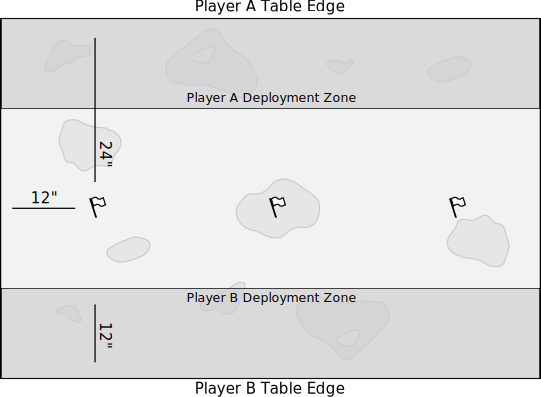
\includegraphics[scale=0.6]{maps/mission1}}

\missionheading{Mission 2: Breakdown}

%\bigskip\centerline{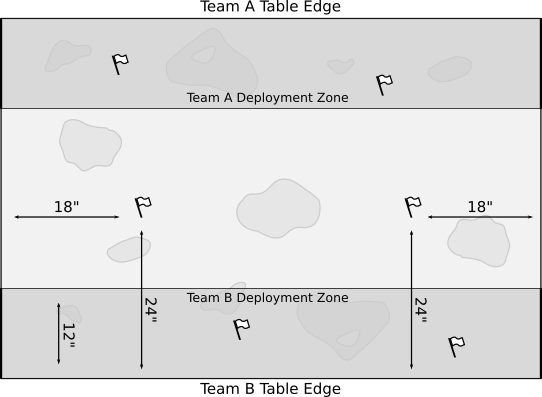
\includegraphics[scale=0.6]{maps/mission2}}

\missionheading{Mission 3: The Maelstrom}

\bigskip\centerline{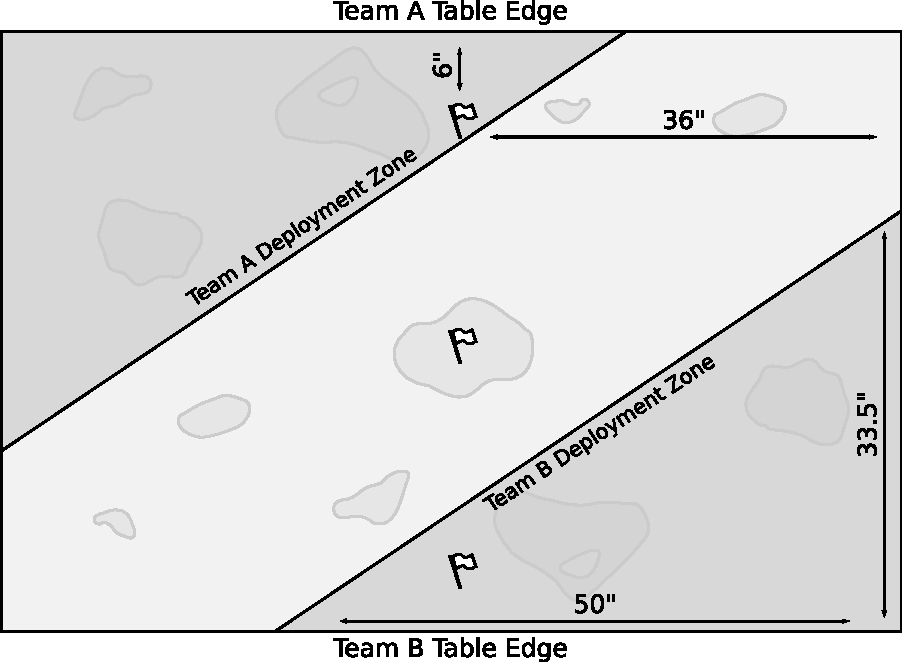
\includegraphics[scale=0.6]{maps/mission3}}

%%----------------------------------------------------------------------
%%----------------------------------------------------------------------
%%----------------------------------------------------------------------
%%----------------------------------------------------------------------
\clearpage
\missiontitle{Mission 1: Madness}

\centerline{\emph{}}

\missionheading{Table Setup}



\bigskip%
After determining deployment zones, place five primary objective
markers: One at the center of the table worth~3 victory points; two
more 18'' from the short table edges and 24'' from the long table
edges worth~2 points each; and two~36'' from the short table edges and
12'' from the long table edges worth~1 point each.

\missionheading{Mission Specific Rules}

The following mission specific rules apply, in addition to those
applied to all missions in this pack.

\missionsubheading{Strike Force.}  All Fast Attack units have the
Obective Secured rule, as defined on page~122 of the rulebook.

%\missionsubheading{Nightfighting.}  All units have Stealth on Turn 1.



\missionheading{Scoring}

This mission is scored by objectives achieved, as follows.

\missionsubheading{Primary Objectives.}  Each primary objective marker
is worth their respective value given above.


\missionsubheading{Secondary Objectives.}

After deployment, both players simultaneously choose and then reveal a
single secondary objective for themselves from the list below.  Any
necessary selections are chosen and then revealed with the objective
unless noted otherwise.  \underline{No more than~6 victory points may
  be earned via any secondary.}

\begin{itemize}
\item \textit{Seize Ground.}  Choose two terrain pieces not in your
  deployment zone.  Do not declare these now, but do secretly record
  your selection unambiguously!  Reveal these at game end and score~3
  victory points for each piece that you control, treating them as
  objective markers.  Note that this means a single unit cannot claim
  both a primary objective marker and a terrain piece simultaneously.

\item \textit{Seek and Destroy.}  Choose and declare a Battlefield
  Role other than Troop.  Score~2 victory points for each enemy unit
  of this role completely destroyed or falling back at the end of the
  game.

\item \textit{Assassinate.}  Score~1 victory point for each opposing
  character model removed as a casualty or falling back at the end of
  the game.  Note that this is not limited to just independent
  characters.
\end{itemize}

\tertiaries

%%----------------------------------------------------------------------
%%----------------------------------------------------------------------
\missiontitle{Mission 2: Slaughter Zone}

\begin{tablesetup}

  \vanguardstrike

\end{tablesetup}

%%----------------------------------------------
\begin{missionrules}

\bigskip
  There are no rules specific to this mission, just those applied to
  all in this packet.

\end{missionrules}

%%----------------------------------------------
\begin{scoring}  
\begin{primaries}
  At game end, each unit that has been eliminated, is falling back, is
  in reserve, or has at most~25\% of its starting models remaining is
  broken.  Earn~2 victory points per quartile if at least 25\%, 50\%,
  and 75\% of the opposing army by units is broken.  Earn~1 victory
  point per quartile if at least 25\%, 50\%, and 75\% of your army is
  not broken.  An additional victory point is earned by the player who
  has had a smaller percentage of the units in their army broken.  If
  one player has been completely eliminated, the opposing player gains
  an additional victory point.  \underline{No more than 9 victory
    points may be earned via this primary objective.}
\end{primaries}

\begin{secondaries}
\interrogation
\seekanddestroy
\chosenground
\majoritycontrol
\end{secondaries}

\end{scoring}

%%----------------------------------------------------------------------
%%----------------------------------------------------------------------
\missiontitle{Mission 3: Battlefield}

\begin{tablesetup}

  \dawnofwar

  \smallskip%
  Place a primary objective marker 16'' x 16'' from each table corner,
  and a fifth at table center.

\end{tablesetup}

%%----------------------------------------------
\begin{missionrules}

  \bigskip%
  There are no rules specific to this mission, just those applied to
  all in this packet.

\end{missionrules}

%%----------------------------------------------
\begin{scoring}  
\begin{primaries}
  Simultaneously with declaring secondary objectives, both players
  choose and declare three of the following primary scoring mechanisms
  for themselves, \underline{earning at most 9 victory points}:

  \begin{enumerate}[label=\Alph*.]\shortlist
  \item Control the primary objective marker at table center at game
    end for~3 victory points.

  \item Choose and declare one of the primary objective markers in
    your opponent's table corners and earn~3 victory points if you
    control it at game end.

  \item Earn~1 victory point at game end for each primary objective
    marker controlled, up to a total of~3 victory points; a marker
    cannot be scored for both this objective and objectives~A or~B.

  \item Earn~3 victory points if at least 25\% of the opposing army by
    units is broken.

  \item Earn~3 victory points if at least 50\% of the opposing army by
    units is broken.

  \item Earn~1 victory point per quartile if at least 25\%, 50\%, and
    75\% of your army is \emph{not} broken.
  \end{enumerate}

  Units are considered broken if at game end they have been
  eliminated, are falling back, are in reserve, or have at most~25\%
  of their starting models remaining.
\end{primaries}

\begin{secondaries}
\assassination
\meatgrinder
\reconnaissance
\breachpoints
\end{secondaries}

\end{scoring}


\end{document}
